\documentclass[a4paper]{article}
% maxwidth is the original width if it is less than linewidth
% otherwise use linewidth (to make sure the graphics do not exceed the margin)
\makeatletter
\def\maxwidth{ %
  \ifdim\Gin@nat@width>\linewidth
    \linewidth
  \else
    \Gin@nat@width
  \fi
}
\makeatother

\usepackage[utf8]{inputenc}
\usepackage{a4wide,paralist}
\usepackage{amsmath, amssymb, xfrac, amsthm}
\usepackage{dsfont}
\usepackage{xcolor}
\usepackage{amsfonts}
\usepackage{graphicx}
\usepackage{hyperref}
\usepackage{bm}
\usepackage{underscore}

% for showing python code blocks
\usepackage{listings}
\lstdefinestyle{pythonstyle}{
    language=Python,
    backgroundcolor=\color[HTML]{F0F0F0},
    commentstyle=\color[HTML]{44515E},
    keywordstyle=\color[HTML]{228A96},
    numberstyle=\color[HTML]{F36E3A},
    stringstyle=\color[HTML]{6BA77F},
    basicstyle=\ttfamily\small,        
    breakatwhitespace=false,          
    breaklines=true,                  
    captionpos=b,                     
    keepspaces=true,                  
    numbers=none,                     
    numbersep=5pt,                   
    showspaces=false,                
    showstringspaces=false,
    showtabs=false,                  
    tabsize=4,
    literate=%
        {0}{{{\color[HTML]{F36E3A}0}}}1
        {1}{{{\color[HTML]{F36E3A}1}}}1
        {2}{{{\color[HTML]{F36E3A}2}}}1
        {3}{{{\color[HTML]{F36E3A}3}}}1
        {4}{{{\color[HTML]{F36E3A}4}}}1
        {5}{{{\color[HTML]{F36E3A}5}}}1
        {6}{{{\color[HTML]{F36E3A}6}}}1
        {7}{{{\color[HTML]{F36E3A}7}}}1
        {8}{{{\color[HTML]{F36E3A}8}}}1
        {9}{{{\color[HTML]{F36E3A}9}}}1
        {e+}{{{\color[HTML]{F36E3A}e+}}}1
        {e-}{{{\color[HTML]{F36E3A}e-}}}1,
}

\lstdefinestyle{rstyle}{
    language=R,
    backgroundcolor=\color[HTML]{F0F0F0},
    commentstyle=\color[HTML]{44515E},
    keywordstyle=\color[HTML]{228A96},
    numberstyle=\color[HTML]{F36E3A},
    stringstyle=\color[HTML]{6BA77F},
    basicstyle=\ttfamily\small,        
    breakatwhitespace=false,          
    breaklines=true,                  
    captionpos=b,                     
    keepspaces=true,                  
    numbers=none,                     
    numbersep=5pt,                   
    showspaces=false,                
    showstringspaces=false,
    showtabs=false,                  
    tabsize=4,
    literate=%
        {0}{{{\color[HTML]{F36E3A}0}}}1
        {1}{{{\color[HTML]{F36E3A}1}}}1
        {2}{{{\color[HTML]{F36E3A}2}}}1
        {3}{{{\color[HTML]{F36E3A}3}}}1
        {4}{{{\color[HTML]{F36E3A}4}}}1
        {5}{{{\color[HTML]{F36E3A}5}}}1
        {6}{{{\color[HTML]{F36E3A}6}}}1
        {7}{{{\color[HTML]{F36E3A}7}}}1
        {8}{{{\color[HTML]{F36E3A}8}}}1
        {9}{{{\color[HTML]{F36E3A}9}}}1
        {e+}{{{\color[HTML]{F36E3A}e+}}}1
        {e-}{{{\color[HTML]{F36E3A}e-}}}1,
    alsoletter ={_},
    otherkeywords = {!,!=,~,$,*,\&,\%/\%,\%*\%,\%\%,<-,<<-},
    morekeywords = {str_extract}
}

\lstset{style=pythonstyle}


% %exercise numbering
\renewcommand{\theenumi}{(\alph{enumi})}
\renewcommand{\theenumii}{\roman{enumii}}
\renewcommand\labelenumi{\theenumi}


\font \sfbold=cmssbx10

\setlength{\oddsidemargin}{0cm} \setlength{\textwidth}{16cm}


\sloppy
\parindent0em
\parskip0.5em
\topmargin-2.3 cm
\textheight25cm
\textwidth17.5cm
\oddsidemargin-0.8cm
\pagestyle{empty}


\newcommand{\kopfaml}[2]{
\hrule
\vspace{.15cm}
\begin{minipage}{\textwidth}
%akwardly i had to put \" here to make it compile correctly
	{\sf\bf Advanced Machine Learning \hfill Exercise sheet #1\\
	 \url{https://slds-lmu.github.io/i2ml/} \hfill #2}
\end{minipage}
\vspace{.05cm}
\hrule
\vspace{1cm}}


\newenvironment{allgemein}
	{\noindent}{\vspace{1cm}}

\newcounter{aufg}
\newenvironment{aufgabe}[1]
	{\refstepcounter{aufg}\textbf{Exercise \arabic{aufg}: #1}\\ \noindent}
	{\vspace{0.5cm}}

\newcounter{loes}
\newenvironment{loesung}[1]
	{\refstepcounter{loes}\textbf{Solution \arabic{loes}: #1}\\\noindent}
	{\bigskip}

\newenvironment{bonusaufgabe}
	{\refstepcounter{aufg}\textbf{Exercise \arabic{aufg}*\footnote{This
	is a bonus exercise.}:}\\ \noindent}
	{\vspace{0.5cm}}

\newenvironment{bonusloesung}
	{\refstepcounter{loes}\textbf{Solution \arabic{loes}*:}\\\noindent}
	{\bigskip}



\begin{document}

\lstset{style=rstyle}


% dependencies: amsmath, amssymb, dsfont
% math spaces
\ifdefined\N
\renewcommand{\N}{\mathds{N}} % N, naturals
\else \newcommand{\N}{\mathds{N}} \fi
\newcommand{\Z}{\mathds{Z}} % Z, integers
\newcommand{\Q}{\mathds{Q}} % Q, rationals
\newcommand{\R}{\mathds{R}} % R, reals
\ifdefined\C
\renewcommand{\C}{\mathds{C}} % C, complex
\else \newcommand{\C}{\mathds{C}} \fi
\newcommand{\continuous}{\mathcal{C}} % C, space of continuous functions
\newcommand{\M}{\mathcal{M}} % machine numbers
\newcommand{\epsm}{\epsilon_m} % maximum error

% counting / finite sets
\newcommand{\setzo}{\{0, 1\}} % set 0, 1
\newcommand{\setmp}{\{-1, +1\}} % set -1, 1
\newcommand{\unitint}{[0, 1]} % unit interval

% basic math stuff
\newcommand{\xt}{\tilde x} % x tilde
\DeclareMathOperator*{\argmax}{arg\,max} % argmax
\DeclareMathOperator*{\argmin}{arg\,min} % argmin
\newcommand{\argminlim}{\mathop{\mathrm{arg\,min}}\limits} % argmax with limits
\newcommand{\argmaxlim}{\mathop{\mathrm{arg\,max}}\limits} % argmin with limits
\newcommand{\sign}{\operatorname{sign}} % sign, signum
\newcommand{\I}{\mathbb{I}} % I, indicator
\newcommand{\order}{\mathcal{O}} % O, order
\newcommand{\bigO}{\mathcal{O}} % Big-O Landau
\newcommand{\littleo}{{o}} % Little-o Landau
\newcommand{\pd}[2]{\frac{\partial{#1}}{\partial #2}} % partial derivative
\newcommand{\floorlr}[1]{\left\lfloor #1 \right\rfloor} % floor
\newcommand{\ceillr}[1]{\left\lceil #1 \right\rceil} % ceiling
\newcommand{\indep}{\perp \!\!\! \perp} % independence symbol

% sums and products
\newcommand{\sumin}{\sum\limits_{i=1}^n} % summation from i=1 to n
\newcommand{\sumim}{\sum\limits_{i=1}^m} % summation from i=1 to m
\newcommand{\sumjn}{\sum\limits_{j=1}^n} % summation from j=1 to p
\newcommand{\sumjp}{\sum\limits_{j=1}^p} % summation from j=1 to p
\newcommand{\sumik}{\sum\limits_{i=1}^k} % summation from i=1 to k
\newcommand{\sumkg}{\sum\limits_{k=1}^g} % summation from k=1 to g
\newcommand{\sumjg}{\sum\limits_{j=1}^g} % summation from j=1 to g
\newcommand{\meanin}{\frac{1}{n} \sum\limits_{i=1}^n} % mean from i=1 to n
\newcommand{\meanim}{\frac{1}{m} \sum\limits_{i=1}^m} % mean from i=1 to n
\newcommand{\meankg}{\frac{1}{g} \sum\limits_{k=1}^g} % mean from k=1 to g
\newcommand{\prodin}{\prod\limits_{i=1}^n} % product from i=1 to n
\newcommand{\prodkg}{\prod\limits_{k=1}^g} % product from k=1 to g
\newcommand{\prodjp}{\prod\limits_{j=1}^p} % product from j=1 to p

% linear algebra
\newcommand{\one}{\bm{1}} % 1, unitvector
\newcommand{\zero}{\mathbf{0}} % 0-vector
\newcommand{\id}{\bm{I}} % I, identity
\newcommand{\diag}{\operatorname{diag}} % diag, diagonal
\newcommand{\trace}{\operatorname{tr}} % tr, trace
\newcommand{\spn}{\operatorname{span}} % span
\newcommand{\scp}[2]{\left\langle #1, #2 \right\rangle} % <.,.>, scalarproduct
\newcommand{\mat}[1]{\begin{pmatrix} #1 \end{pmatrix}} % short pmatrix command
\newcommand{\Amat}{\mathbf{A}} % matrix A
\newcommand{\Deltab}{\mathbf{\Delta}} % error term for vectors

% basic probability + stats
\renewcommand{\P}{\mathds{P}} % P, probability
\newcommand{\E}{\mathds{E}} % E, expectation
\newcommand{\var}{\mathsf{Var}} % Var, variance
\newcommand{\cov}{\mathsf{Cov}} % Cov, covariance
\newcommand{\corr}{\mathsf{Corr}} % Corr, correlation
\newcommand{\normal}{\mathcal{N}} % N of the normal distribution
\newcommand{\iid}{\overset{i.i.d}{\sim}} % dist with i.i.d superscript
\newcommand{\distas}[1]{\overset{#1}{\sim}} % ... is distributed as ...

% machine learning
\newcommand{\Xspace}{\mathcal{X}} % X, input space
\newcommand{\Yspace}{\mathcal{Y}} % Y, output space
\newcommand{\Zspace}{\mathcal{Z}} % Space of sampled datapoints ! Also defined identically in ml-online.tex !
\newcommand{\nset}{\{1, \ldots, n\}} % set from 1 to n
\newcommand{\pset}{\{1, \ldots, p\}} % set from 1 to p
\newcommand{\gset}{\{1, \ldots, g\}} % set from 1 to g
\newcommand{\Pxy}{\mathbb{P}_{xy}} % P_xy
\newcommand{\Exy}{\mathbb{E}_{xy}} % E_xy: Expectation over random variables xy
\newcommand{\xv}{\mathbf{x}} % vector x (bold)
\newcommand{\xtil}{\tilde{\mathbf{x}}} % vector x-tilde (bold)
\newcommand{\yv}{\mathbf{y}} % vector y (bold)
\newcommand{\xy}{(\xv, y)} % observation (x, y)
\newcommand{\xvec}{\left(x_1, \ldots, x_p\right)^\top} % (x1, ..., xp)
\newcommand{\Xmat}{\mathbf{X}} % Design matrix
\newcommand{\allDatasets}{\mathds{D}} % The set of all datasets
\newcommand{\allDatasetsn}{\mathds{D}_n}  % The set of all datasets of size n
\newcommand{\D}{\mathcal{D}} % D, data
\newcommand{\Dn}{\D_n} % D_n, data of size n
\newcommand{\Dtrain}{\mathcal{D}_{\text{train}}} % D_train, training set
\newcommand{\Dtest}{\mathcal{D}_{\text{test}}} % D_test, test set
\newcommand{\xyi}[1][i]{\left(\xv^{(#1)}, y^{(#1)}\right)} % (x^i, y^i), i-th observation
\newcommand{\Dset}{\left( \xyi[1], \ldots, \xyi[n]\right)} % {(x1,y1)), ..., (xn,yn)}, data
\newcommand{\defAllDatasetsn}{(\Xspace \times \Yspace)^n} % Def. of the set of all datasets of size n
\newcommand{\defAllDatasets}{\bigcup_{n \in \N}(\Xspace \times \Yspace)^n} % Def. of the set of all datasets
\newcommand{\xdat}{\left\{ \xv^{(1)}, \ldots, \xv^{(n)}\right\}} % {x1, ..., xn}, input data
\newcommand{\ydat}{\left\{ \yv^{(1)}, \ldots, \yv^{(n)}\right\}} % {y1, ..., yn}, input data
\newcommand{\yvec}{\left(y^{(1)}, \hdots, y^{(n)}\right)^\top} % (y1, ..., yn), vector of outcomes
\renewcommand{\xi}[1][i]{\xv^{(#1)}} % x^i, i-th observed value of x
\newcommand{\yi}[1][i]{y^{(#1)}} % y^i, i-th observed value of y
\newcommand{\xivec}{\left(x^{(i)}_1, \ldots, x^{(i)}_p\right)^\top} % (x1^i, ..., xp^i), i-th observation vector
\newcommand{\xj}{\xv_j} % x_j, j-th feature
\newcommand{\xjvec}{\left(x^{(1)}_j, \ldots, x^{(n)}_j\right)^\top} % (x^1_j, ..., x^n_j), j-th feature vector
\newcommand{\phiv}{\mathbf{\phi}} % Basis transformation function phi
\newcommand{\phixi}{\mathbf{\phi}^{(i)}} % Basis transformation of xi: phi^i := phi(xi)

%%%%%% ml - models general
\newcommand{\lamv}{\bm{\lambda}} % lambda vector, hyperconfiguration vector
\newcommand{\Lam}{\bm{\Lambda}}	 % Lambda, space of all hpos
% Inducer / Inducing algorithm
\newcommand{\preimageInducer}{\left(\defAllDatasets\right)\times\Lam} % Set of all datasets times the hyperparameter space
\newcommand{\preimageInducerShort}{\allDatasets\times\Lam} % Set of all datasets times the hyperparameter space
% Inducer / Inducing algorithm
\newcommand{\ind}{\mathcal{I}} % Inducer, inducing algorithm, learning algorithm

% continuous prediction function f
\newcommand{\ftrue}{f_{\text{true}}}  % True underlying function (if a statistical model is assumed)
\newcommand{\ftruex}{\ftrue(\xv)} % True underlying function (if a statistical model is assumed)
\newcommand{\fx}{f(\xv)} % f(x), continuous prediction function
\newcommand{\fdomains}{f: \Xspace \rightarrow \R^g} % f with domain and co-domain
\newcommand{\Hspace}{\mathcal{H}} % hypothesis space where f is from
\newcommand{\fbayes}{f^{\ast}} % Bayes-optimal model
\newcommand{\fxbayes}{f^{\ast}(\xv)} % Bayes-optimal model
\newcommand{\fkx}[1][k]{f_{#1}(\xv)} % f_j(x), discriminant component function
\newcommand{\fh}{\hat{f}} % f hat, estimated prediction function
\newcommand{\fxh}{\fh(\xv)} % fhat(x)
\newcommand{\fxt}{f(\xv ~|~ \thetab)} % f(x | theta)
\newcommand{\fxi}{f\left(\xv^{(i)}\right)} % f(x^(i))
\newcommand{\fxih}{\hat{f}\left(\xv^{(i)}\right)} % f(x^(i))
\newcommand{\fxit}{f\left(\xv^{(i)} ~|~ \thetab\right)} % f(x^(i) | theta)
\newcommand{\fhD}{\fh_{\D}} % fhat_D, estimate of f based on D
\newcommand{\fhDtrain}{\fh_{\Dtrain}} % fhat_Dtrain, estimate of f based on D
\newcommand{\fhDnlam}{\fh_{\Dn, \lamv}} %model learned on Dn with hp lambda
\newcommand{\fhDlam}{\fh_{\D, \lamv}} %model learned on D with hp lambda
\newcommand{\fhDnlams}{\fh_{\Dn, \lamv^\ast}} %model learned on Dn with optimal hp lambda
\newcommand{\fhDlams}{\fh_{\D, \lamv^\ast}} %model learned on D with optimal hp lambda

% discrete prediction function h
\newcommand{\hx}{h(\xv)} % h(x), discrete prediction function
\newcommand{\hh}{\hat{h}} % h hat
\newcommand{\hxh}{\hat{h}(\xv)} % hhat(x)
\newcommand{\hxt}{h(\xv | \thetab)} % h(x | theta)
\newcommand{\hxi}{h\left(\xi\right)} % h(x^(i))
\newcommand{\hxit}{h\left(\xi ~|~ \thetab\right)} % h(x^(i) | theta)
\newcommand{\hbayes}{h^{\ast}} % Bayes-optimal classification model
\newcommand{\hxbayes}{h^{\ast}(\xv)} % Bayes-optimal classification model

% yhat
\newcommand{\yh}{\hat{y}} % yhat for prediction of target
\newcommand{\yih}{\hat{y}^{(i)}} % yhat^(i) for prediction of ith targiet
\newcommand{\resi}{\yi- \yih}

% theta
\newcommand{\thetah}{\hat{\theta}} % theta hat
\newcommand{\thetab}{\bm{\theta}} % theta vector
\newcommand{\thetabh}{\bm{\hat\theta}} % theta vector hat
\newcommand{\thetat}[1][t]{\thetab^{[#1]}} % theta^[t] in optimization
\newcommand{\thetatn}[1][t]{\thetab^{[#1 +1]}} % theta^[t+1] in optimization
\newcommand{\thetahDnlam}{\thetabh_{\Dn, \lamv}} %theta learned on Dn with hp lambda
\newcommand{\thetahDlam}{\thetabh_{\D, \lamv}} %theta learned on D with hp lambda
\newcommand{\mint}{\min_{\thetab \in \Theta}} % min problem theta
\newcommand{\argmint}{\argmin_{\thetab \in \Theta}} % argmin theta

% densities + probabilities
% pdf of x
\newcommand{\pdf}{p} % p
\newcommand{\pdfx}{p(\xv)} % p(x)
\newcommand{\pixt}{\pi(\xv~|~ \thetab)} % pi(x|theta), pdf of x given theta
\newcommand{\pixit}[1][i]{\pi\left(\xi[#1] ~|~ \thetab\right)} % pi(x^i|theta), pdf of x given theta
\newcommand{\pixii}[1][i]{\pi\left(\xi[#1]\right)} % pi(x^i), pdf of i-th x

% pdf of (x, y)
\newcommand{\pdfxy}{p(\xv,y)} % p(x, y)
\newcommand{\pdfxyt}{p(\xv, y ~|~ \thetab)} % p(x, y | theta)
\newcommand{\pdfxyit}{p\left(\xi, \yi ~|~ \thetab\right)} % p(x^(i), y^(i) | theta)

% pdf of x given y
\newcommand{\pdfxyk}[1][k]{p(\xv | y= #1)} % p(x | y = k)
\newcommand{\lpdfxyk}[1][k]{\log p(\xv | y= #1)} % log p(x | y = k)
\newcommand{\pdfxiyk}[1][k]{p\left(\xi | y= #1 \right)} % p(x^i | y = k)

% prior probabilities
\newcommand{\pik}[1][k]{\pi_{#1}} % pi_k, prior
\newcommand{\lpik}[1][k]{\log \pi_{#1}} % log pi_k, log of the prior
\newcommand{\pit}{\pi(\thetab)} % Prior probability of parameter theta

% posterior probabilities
\newcommand{\post}{\P(y = 1 ~|~ \xv)} % P(y = 1 | x), post. prob for y=1
\newcommand{\postk}[1][k]{\P(y = #1 ~|~ \xv)} % P(y = k | y), post. prob for y=k
\newcommand{\pidomains}{\pi: \Xspace \rightarrow \unitint} % pi with domain and co-domain
\newcommand{\pibayes}{\pi^{\ast}} % Bayes-optimal classification model
\newcommand{\pixbayes}{\pi^{\ast}(\xv)} % Bayes-optimal classification model
\newcommand{\pix}{\pi(\xv)} % pi(x), P(y = 1 | x)
\newcommand{\piv}{\bm{\pi}} % pi, bold, as vector
\newcommand{\pikx}[1][k]{\pi_{#1}(\xv)} % pi_k(x), P(y = k | x)
\newcommand{\pikxt}[1][k]{\pi_{#1}(\xv ~|~ \thetab)} % pi_k(x | theta), P(y = k | x, theta)
\newcommand{\pixh}{\hat \pi(\xv)} % pi(x) hat, P(y = 1 | x) hat
\newcommand{\pikxh}[1][k]{\hat \pi_{#1}(\xv)} % pi_k(x) hat, P(y = k | x) hat
\newcommand{\pixih}{\hat \pi(\xi)} % pi(x^(i)) with hat
\newcommand{\pikxih}[1][k]{\hat \pi_{#1}(\xi)} % pi_k(x^(i)) with hat
\newcommand{\pdfygxt}{p(y ~|~\xv, \thetab)} % p(y | x, theta)
\newcommand{\pdfyigxit}{p\left(\yi ~|~\xi, \thetab\right)} % p(y^i |x^i, theta)
\newcommand{\lpdfygxt}{\log \pdfygxt } % log p(y | x, theta)
\newcommand{\lpdfyigxit}{\log \pdfyigxit} % log p(y^i |x^i, theta)

% probababilistic
\newcommand{\bayesrulek}[1][k]{\frac{\P(\xv | y= #1) \P(y= #1)}{\P(\xv)}} % Bayes rule
\newcommand{\muk}{\bm{\mu_k}} % mean vector of class-k Gaussian (discr analysis)

% residual and margin
\newcommand{\eps}{\epsilon} % residual, stochastic
\newcommand{\epsi}{\epsilon^{(i)}} % epsilon^i, residual, stochastic
\newcommand{\epsh}{\hat{\epsilon}} % residual, estimated
\newcommand{\yf}{y \fx} % y f(x), margin
\newcommand{\yfi}{\yi \fxi} % y^i f(x^i), margin
\newcommand{\Sigmah}{\hat \Sigma} % estimated covariance matrix
\newcommand{\Sigmahj}{\hat \Sigma_j} % estimated covariance matrix for the j-th class

% ml - loss, risk, likelihood
\newcommand{\Lyf}{L\left(y, f\right)} % L(y, f), loss function
\newcommand{\Lypi}{L\left(y, \pi\right)} % L(y, pi), loss function
\newcommand{\Lxy}{L\left(y, \fx\right)} % L(y, f(x)), loss function
\newcommand{\Lxyi}{L\left(\yi, \fxi\right)} % loss of observation
\newcommand{\Lxyt}{L\left(y, \fxt\right)} % loss with f parameterized
\newcommand{\Lxyit}{L\left(\yi, \fxit\right)} % loss of observation with f parameterized
\newcommand{\Lxym}{L\left(\yi, f\left(\bm{\tilde{x}}^{(i)} ~|~ \thetab\right)\right)} % loss of observation with f parameterized
\newcommand{\Lpixy}{L\left(y, \pix\right)} % loss in classification
\newcommand{\Lpiv}{L\left(y, \piv\right)} % loss in classification
\newcommand{\Lpixyi}{L\left(\yi, \pixii\right)} % loss of observation in classification
\newcommand{\Lpixyt}{L\left(y, \pixt\right)} % loss with pi parameterized
\newcommand{\Lpixyit}{L\left(\yi, \pixit\right)} % loss of observation with pi parameterized
\newcommand{\Lhxy}{L\left(y, \hx\right)} % L(y, h(x)), loss function on discrete classes
\newcommand{\Lr}{L\left(r\right)} % L(r), loss defined on residual (reg) / margin (classif)
\newcommand{\lone}{|y - \fx|} % L1 loss
\newcommand{\ltwo}{\left(y - \fx\right)^2} % L2 loss
\newcommand{\lbernoullimp}{\ln(1 + \exp(-y \cdot \fx))} % Bernoulli loss for -1, +1 encoding
\newcommand{\lbernoullizo}{- y \cdot \fx + \log(1 + \exp(\fx))} % Bernoulli loss for 0, 1 encoding
\newcommand{\lcrossent}{- y \log \left(\pix\right) - (1 - y) \log \left(1 - \pix\right)} % cross-entropy loss
\newcommand{\lbrier}{\left(\pix - y \right)^2} % Brier score
\newcommand{\risk}{\mathcal{R}} % R, risk
\newcommand{\riskbayes}{\mathcal{R}^\ast}
\newcommand{\riskf}{\risk(f)} % R(f), risk
\newcommand{\riskdef}{\E_{y|\xv}\left(\Lxy \right)} % risk def (expected loss)
\newcommand{\riskt}{\mathcal{R}(\thetab)} % R(theta), risk
\newcommand{\riske}{\mathcal{R}_{\text{emp}}} % R_emp, empirical risk w/o factor 1 / n
\newcommand{\riskeb}{\bar{\mathcal{R}}_{\text{emp}}} % R_emp, empirical risk w/ factor 1 / n
\newcommand{\riskef}{\riske(f)} % R_emp(f)
\newcommand{\risket}{\mathcal{R}_{\text{emp}}(\thetab)} % R_emp(theta)
\newcommand{\riskr}{\mathcal{R}_{\text{reg}}} % R_reg, regularized risk
\newcommand{\riskrt}{\mathcal{R}_{\text{reg}}(\thetab)} % R_reg(theta)
\newcommand{\riskrf}{\riskr(f)} % R_reg(f)
\newcommand{\riskrth}{\hat{\mathcal{R}}_{\text{reg}}(\thetab)} % hat R_reg(theta)
\newcommand{\risketh}{\hat{\mathcal{R}}_{\text{emp}}(\thetab)} % hat R_emp(theta)
\newcommand{\LL}{\mathcal{L}} % L, likelihood
\newcommand{\LLt}{\mathcal{L}(\thetab)} % L(theta), likelihood
\newcommand{\LLtx}{\mathcal{L}(\thetab | \xv)} % L(theta|x), likelihood
\newcommand{\logl}{\ell} % l, log-likelihood
\newcommand{\loglt}{\logl(\thetab)} % l(theta), log-likelihood
\newcommand{\logltx}{\logl(\thetab | \xv)} % l(theta|x), log-likelihood
\newcommand{\errtrain}{\text{err}_{\text{train}}} % training error
\newcommand{\errtest}{\text{err}_{\text{test}}} % test error
\newcommand{\errexp}{\overline{\text{err}_{\text{test}}}} % avg training error

% lm
\newcommand{\thx}{\thetab^\top \xv} % linear model
\newcommand{\olsest}{(\Xmat^\top \Xmat)^{-1} \Xmat^\top \yv} % OLS estimator in LM


\kopfaml{11}{Multitarget Learning}

\newcommand{\ba}{\mathbf{a}}

\loesung{Multivariate Regression}{

Consider the multivariate regression setting on $\Xspace \subset \R^p$ without target features, i.e., $\Yspace=\R$ and $\mathcal{T} = \{1,\ldots,m\}.$	
Furthermore, consider the approach of learning a (simple) linear model $f_j(\xv) = \ba_j^\top \xv$ for each target $j$ independently.
For this purpose, we would face the following optimization problem:
\begin{equation*}	\label{eq:multiridge}
	\min_A \|Y - \Xmat A \|^2_F,		
\end{equation*}
where  $ \| B \|^2_F  = \sqrt{ \sum_{i=1}^n \sum_{j=1}^m B_{i,j}^2 } $ is the Frobenius norm for a matrix $B \in \R^{n \times m}$ and 
%		
\begin{equation*} \label{eq:notation}
    \Xmat = \begin{bmatrix} (\xv^{(1)} )^\top \\ \vdots \\ (\xv^{(n)})^\top \end{bmatrix}, \qquad A = [\ba_1 \quad \cdots \quad \ba_m] \,, \qquad Y = \begin{bmatrix} \yv^{(1)}\\ \vdots \\ \yv^{(n)} \end{bmatrix}.
\end{equation*}

\begin{enumerate}
	\item Show that $\hat A = (\Xmat^\top \Xmat)^{-1} \Xmat^\top Y$ is the optimal solution in this case (provided that $\Xmat^\top \Xmat$ is invertible).
	
	\textbf{Solution:}
	
	Note that for a matrix $B = (\bm{b}_1 \ldots \bm{b}_m) \in \R^{n\times m},$ it holds that
	\begin{align*} 
		\| B \|^2_F   
	 	=  \sum_{i=1}^n \sum_{j=1}^m B_{i,j}^2 
		=  \sum_{j=1}^m \sum_{i=1}^n B_{i,j}^2 
		&=  \sum_{j=1}^m \bm{b}_j^\top \bm{b}_j. 
	\end{align*}
	Thus, the function $f(A)=\|Y - \Xmat A \|^2_F$ we want to minimize can be written as
	\begin{align*}
		\|Y - \Xmat A \|^2_F 
		&= \sum_{j=1}^m (\bm{y}_j -\Xmat \bm{a}_j)^\top(\bm{y}_j -\Xmat \bm{a}_j) \\
		&= \sum_{j=1}^m \bm{y}_j^\top\bm{y}_j - 2 \bm{y}_j^\top \Xmat \bm{a}_j + \bm{a}_j^\top \Xmat^\top  \Xmat \bm{a}_j,
	\end{align*}
	where $\bm{y}_j$ is the $j$-th column of $Y.$
	Therefore, we can write $f(A) = \sum_{j=1}^m f_j(\ba_j),$ where 
	$$	f_j(\ba) = 	\bm{y}_j^\top\bm{y}_j - 2 \bm{y}_j^\top \Xmat \bm{a} + \bm{a}^\top \Xmat^\top  \Xmat \bm{a}	$$
	and we can minimize each $f_j$ separately (w.r.t.\ to $\ba_j$).
	We compute the gradient of $f_j$ and set it to $\bm{0}$ and solve w.r.t.\ $\ba:$
	\begin{align*}
		\nabla f_j(\ba) 
		&= - 2 \bm{y}_j^\top \Xmat  + 2 \Xmat^\top  \Xmat \bm{a} \stackrel{!}{=} \bm{0} \\
		&\Leftrightarrow \ba = (\Xmat^\top \Xmat)^{-1} \Xmat^\top \bm{y}_j.
	\end{align*}
	We check that this is indeed a minimum, by checking that the Hessian matrix is positive semi-definite:
	The Hessian matrix is
    \begin{align*}	
        \nabla \nabla^\top f_j(\ba) 		
        &=   2 \Xmat^\top  \Xmat.		
	\end{align*}
	It is positive semi-definite, since for any $\bm{z}\in \R^p$ it holds that
	\begin{align*}
		\bm{z}^\top (2 \Xmat^\top  \Xmat) \bm{z} 
		= 2 \bm{z}^\top  \Xmat^\top  \Xmat  \bm{z} 
		= 	2   (\Xmat  \bm{z})^\top \Xmat  \bm{z} 
		= 2 \| \Xmat  \bm{z} \|_2^2 \geq 0.
	\end{align*}
	Consequently, the minimizer of $f_j$ is $\hat{\ba}_j= (\Xmat^\top \Xmat)^{-1} \Xmat^\top \bm{y}_j,$ so that the minimizer of $f$ is 
 
	$$	\hat{A} = (\hat{\ba}_1 ~ \ldots ~ \hat{\ba}_m) = \left(	(\Xmat^\top \Xmat)^{-1} \Xmat^\top \bm{y}_1 ~ \ldots ~ (\Xmat^\top \Xmat)^{-1} \Xmat^\top \bm{y}_m		\right) = (\Xmat^\top \Xmat)^{-1} \Xmat^\top Y.	$$
	In particular, the gradient of $f$ w.r.t.\ matrix $A=(\ba_1 ~ \ldots ~ \ba_m)$ is 
	\begin{align*}
		\nabla f(A) 	
		&= ( \nabla f_1(\ba_1) ~ \ldots ~ \nabla f_m(\ba_m) )  \\
		&= \left( - 2 \bm{y}_1^\top \Xmat  + 2 \Xmat^\top  \Xmat \bm{a}_1 \quad \ldots \quad - 2 \bm{y}_m^\top \Xmat  + 2 \Xmat^\top  \Xmat \bm{a}_m\right) \\
		&= -2Y^\top \Xmat  + 2 \Xmat^\top  \Xmat A.
	\end{align*}
	Hence, a gradient descent routine with (fixed) step size $\alpha$ for $f$ would iterate as follows:
	\begin{align*}	
		\hat A \leftarrow \hat A - 2 \alpha \left( -Y^\top \Xmat  +  \Xmat^\top  \Xmat \hat A \right).	
	\end{align*}
	\item Assume that the data $(\xi,\yv^{(i)}) \in \Xspace \times \Yspace^m$ is generated\footnote{Of course, in an iid fashion and the $\xv$'s are independent of the $\bm{\eps}$'s.} according to the following statistical model
	$$	(y_1,\ldots,y_m) =	\yv = (\xi)^\top A^* + \bm{\eps}^\top,		$$
	where $A^* \in \R^{p\times m}$ and $\bm{\eps} \sim \normal(\bm{0},\bm{\Sigma}).$
	Show that the maximum likelihood estimate for $A^*$ coincides with the estimate in (a). 
	
	\textbf{Solution:}
	
	Under the statistical model it holds that $\yv^{(i)}~|~\xi \sim \normal\left(	(\xi)^\top A^*, \bm{\Sigma}	\right),$ i.e.\footnote{Note that $\yv^{(i)} - (\xi)^\top A^* $ is a row vector.},
	\begin{align}\label{def_distr}
		p(\yv^{(i)}~|~\xi,A^*) 
		&= (2\pi)^{-m/2} |\bm{\Sigma}|^{-1/2} \, \exp\left[	-\frac12 (\yv^{(i)} - (\xi)^\top A^* )	\bm{\Sigma}^{-1} (\yv^{(i)} - (\xi)^\top A^* )^\top	\right] \notag \\
		&\propto \exp\left[	-\frac12 \left(\yv^{(i)} - (\xi)^\top A^* \right)	\bm{\Sigma}^{-1} \left(\yv^{(i)} - (\xi)^\top A^* \right)^\top	\right] .
	\end{align}
	So the log-likelihood for $A$ is
	\begin{align*}
		l(A~|~\D) 
		&= \log\left(	\prod_{i=1}^n 		p(\yv^{(i)}~|~\xi,A)	\right) \\
		&\propto \log\left(	 	\exp\left[	-\frac12 \sum_{i=1}^n \left(\yv^{(i)} - (\xi)^\top A \right)	\bm{\Sigma}^{-1} \left(\yv^{(i)} - (\xi)^\top A \right)^\top	\right]	\right) \\
		&= 	-\sum_{i=1}^n  \left(\yv^{(i)} - (\xi)^\top A \right)	\bm{\Sigma}^{-1} \left(\yv^{(i)} - (\xi)^\top A \right)^\top.		 
	\end{align*}
	So, we want to maximize the function 
	\begin{align*}
		g(A) 
		&= 	-\sum_{i=1}^n  \left(\yv^{(i)} - (\xi)^\top A \right)	\bm{\Sigma}^{-1} \left(\yv^{(i)} - (\xi)^\top A \right)^\top \\
		&= 	-\sum_{i=1}^n  \yv^{(i)} \bm{\Sigma}^{-1} (\yv^{(i)})^\top  
		- 2 (\xi)^\top A \bm{\Sigma}^{-1} (\yv^{(i)})^\top 
		+ (\xi)^\top A	\bm{\Sigma}^{-1}  A^\top \xi.	
	\end{align*}
	We compute the gradient of $g$ and set it to $\bm{0}_{p\times m}$ and solve w.r.t.\ $A:$
	\begin{align*}
		\nabla g(A) 
		&= 	\sum_{i=1}^n   2 \xi \yv^{(i)}   \bm{\Sigma}^{-1}
		- 2   \xi	(\xi)^\top  A \bm{\Sigma}^{-1}   \stackrel{!}{=} \bm{0}_{p\times m} \\
		%		
		&\Leftrightarrow 	\Xmat^\top Y  \bm{\Sigma}^{-1}
		-   \Xmat^\top \Xmat  A \bm{\Sigma}^{-1}   \stackrel{!}{=} \bm{0}_{p\times m} \\
		&\Leftrightarrow A = (\Xmat^\top \Xmat)^{-1} \Xmat^\top Y,	
	\end{align*}
	where we used for computing the gradient that 
	\begin{align*}
		&\frac{\partial \bm{z}^\top \bm{B} \tilde{\bm{z}} }{\partial  \bm{B} } = \bm{z} \tilde{\bm{z}}^\top, \qquad \forall \bm{z}\in\R^n,\tilde{\bm{z}}\in \R^{m}, \bm{B}\in\R^{n \times m}, \\
		&\frac{\partial \bm{z}^\top \bm{B} \bm{C} \bm{B}^\top \tilde{\bm{z}} }{\partial  \bm{B} } 
		= 2 \bm{z} \tilde{\bm{z}}^\top \bm{B} \bm{C}^\top  , \qquad \forall \bm{z}\in\R^n,\tilde{\bm{z}}\in \R^{m}, \bm{B}\in\R^{n \times m}, \bm{C} \in \R^{n \times n}.
	\end{align*}
	Moreover, any matrix product $\Xmat^\top Y$ can be written as the sum of outer products of the column and row vectors: $ \sum_{i=1}^n    \xi \yv^{(i)}.$
	Thus, the MLE coincides with the OLS in (a).		
	\item Write a function implementing a gradient descent routine for the optimization of this linear model.
	 \item Run a small simulation study by creating 20 data sets as indicated below and test different step sizes $\alpha$ (fixed across iterations) against each other and against the state-of-the-art routine for linear models (in R, using the function \texttt{lm}, in Python, e.g., \texttt{sklearn.linear\_model.LinearRegression}).
  \begin{itemize}
    \item Compare the difference in the estimated parameter matrices $\hat A$ using the mean squared error, i.e., 
    $$ \frac{1}{m\cdot p} \sum_{i=1}^p \sum_{j=1}^m (\ba^{*}_{i,j}-\hat{\ba}_{i,j})^2$$ 
    and summarize the difference over all 100 simulation repetitions.
    \item Compare the estimation also with the James-Stein estimate of $A^*$, which is given by 
	$$  A^{JS} = \left(  \ba_1^{JS} \ldots \ba_m^{JS}  \right),$$
	where $$  \ba_j^{JS} = \left (1 - \frac{(m-2)\sigma^2}{n\|\hat{\ba}_j - \ba_j^* \|^2_2} \right )  (\hat{\ba}_j - \ba_j^*) + \ba_j^*, \quad j=1,\ldots,m.$$
	and $\hat{\ba}_j$ is the MLE for the $j$th target parameter.
    \end{itemize}

\begin{lstlisting}
#' @param step_size the step_size in each iteration 
#' @param X the feature input matrix X 
#' @param Y the score matrix Y 
#' @param A the parameter matrix 
#' @param eps a small constant measuring the changes in each update step. 
#' Stop the algorithm if the estimated model parameters do not change
#' more than eps.

#' @return a set of optimal parameter matrix A

gradient_descent <- function(
                        step_size, 
                        X, 
                        Y, 
                        A = matrix(rep(0,ncol(X)*m),ncol=m),
                        eps = 1e-8){

    change <- 1 # something larger eps

    XtX <- crossprod(X) 
    XtY <- crossprod(X,Y)
    while(sum(abs(change)) > eps) {
        # Use standard gradient descent:
        change <- + step_size * (XtY - XtX%*%A)
        # update A in the end 
        A <- A + change
    }
    return(A)
}

# make it all reproducible 
set.seed(123)

# settings 
n <- 10000 
p <- 100

m <- 6 
nr_sims <- 20

# define mse 
mse <- function(x,y) mean((x-y)^2)

# create data (only once)
X <- matrix(rnorm(n*p), ncol=p)
A_truth <- matrix(runif(p*m, -2, 2),ncol=m) 
f_truth <- X%*%A_truth

# create result object 
result_list <- vector("list", nr_sims)

js_estimate <- function(A,A_truth) { 
    A_JS = A
    for(i in 1:ncol(A)) {

        A_JS[,i]= (1-4*(m-2)/(n*sum((A[,i]-A_truth[,i])^2)))* (A[,i]-A_truth[,i])+A_truth[,i]
    }
    A_JS
}

for(sim_nr in seq_len(nr_sims)){
    # create response
    Y <- f_truth + rnorm(n*m, sd = 2)

    time_lm <- system.time( coef_lm <- coef(lm(Y~-1+X)) )["elapsed"]

    time_js <- system.time( 
                coef_js <- js_estimate(coef_lm,A_truth) )["elapsed"] 
    time_js = time_js + time_lm

    time_gd_1 <- system.time(
                    coef_gd_1 <- gradient_descent(
                        step_size = 0.0001, 
                        X = X, 
                        Y = Y)
                )["elapsed"]

    time_gd_2 <- system.time( 
                    coef_gd_2 <- gradient_descent(
                        step_size = 0.00005, 
                        X = X, 
                        Y = Y)
                )["elapsed"]

    mse_lm <- mse(coef_lm, A_truth) 
    mse_js <- mse(coef_js, A_truth) 
    mse_gd_1 <- mse(coef_gd_1, A_truth) 
    mse_gd_2 <- mse(coef_gd_2, A_truth)

    # save results in list (performance, time) 
    result_list[[sim_nr]] <- data.frame(
                                mse_lm = mse_lm, 
                                mse_js = mse_js, 
                                mse_gd_1 = mse_gd_1,
                                mse_gd_2 = mse_gd_2, 
                                time_lm = time_lm, 
                                time_js = time_js, 
                                time_gd_1 = time_gd_1, 
                                time_gd_2 = time_gd_2)
}

library(ggplot2) 
library(dplyr) 
library(tidyr)

do.call("rbind", result_list) %>% 
    gather() %>%
    mutate(what = ifelse(grepl("mse", key), "MSE", "Time"),
        algorithm = gsub("(mse|time)\\ _(.*)","\\2", key)) %>%
    ggplot(aes(x = algorithm, y = value)) + geom_boxplot() + theme_bw() + 
    facet_wrap(~ what, scales = "free")
\end{lstlisting}

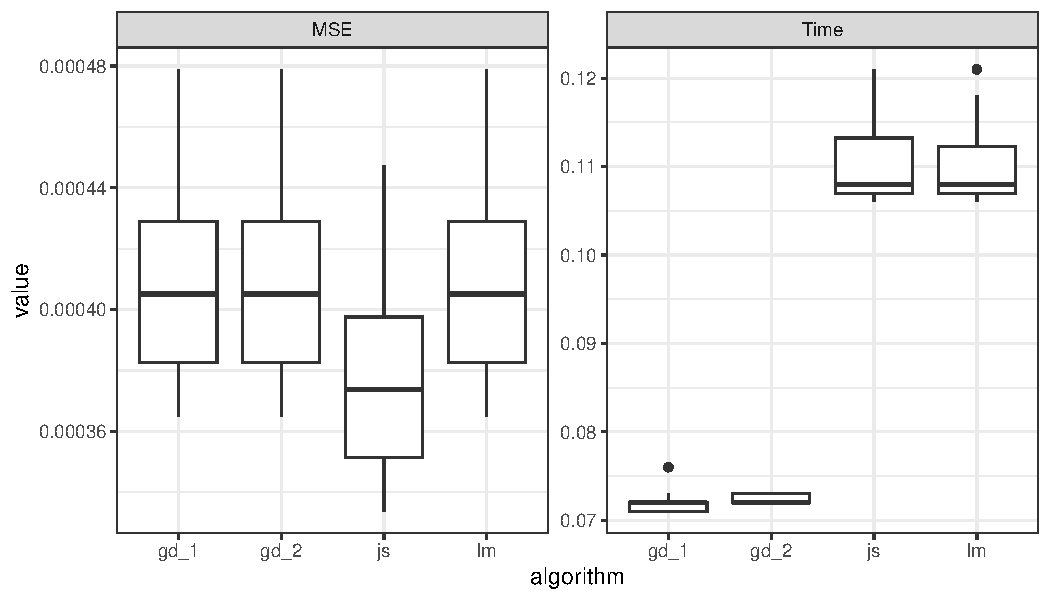
\includegraphics[width=\maxwidth]{figure/unnamed-chunk-3-1}

\end{enumerate}

}


\end{document}